\documentclass{article}
\usepackage{graphicx}
\usepackage{subcaption}
\usepackage{cleveref}
\usepackage{geometry}
\usepackage{tikz}
\def\checkmark{\tikz\fill[scale=0.4](0,.35) -- (.25,0) -- (1,.7) -- (.25,.15) -- cycle;}
\usepackage[font=small,skip=0pt]{caption}
\geometry{legalpaper, margin=1in}

\begin{document}

\textbf{problem 1.}

\vspace{\baselineskip}
\textit{question 1.1.}

population of interest: Time Magazine articles contributed by FZ.

population quantity of interest: the number of Time Magazine articles contributed by FZ.

sampling units: article

\vspace{\baselineskip}
\textit{question 1.2.}

The average and the variance of the number of times that the word \textbf{however} being used \textbf{per article}, the average and the variance of the number of times that the word \textbf{however} being used \textbf{per sentence}.

\vspace{\baselineskip}
\textit{question 1.3.}

\begin{table}[h!]
  \begin{center}
    \begin{tabular}{| c | c | c |}
      \hline
      & varibale & constant \\
      \hline
      observed& \checkmark &  \\
      \hline
      unknown &  &  \\
      \hline
    \end{tabular}
  \end{center}
  \caption{\textit{X\textsubscript{i}, ..., X\textsubscript{n}}}
\end{table}

\begin{table}[h!]
  \begin{center}
    \begin{tabular}{| c | c | c |}
      \hline
      & varibale & constant \\
      \hline
      observed&  & \checkmark \\
      \hline
      unknown &  & \\
      \hline
    \end{tabular}
  \end{center}
  \caption{\textit{x\textsubscript{i}, ..., x\textsubscript{n}}}
\end{table}


\begin{table}[h!]
  \begin{center}
    \begin{tabular}{| c | c | c |}
      \hline
      & varibale & constant \\
      \hline
      observed&  &  \\
      \hline
      unknown & & \checkmark\\
      \hline
    \end{tabular}
  \end{center}
  \caption{\textit{$\lambda$}}
\end{table}

\begin{table}[h!]
  \begin{center}
    \begin{tabular}{| c | c | c |}
      \hline
      & varibale & constant \\
      \hline
      observed&  & \checkmark \\
      \hline
      unknown &  &  \\
      \hline
    \end{tabular}
  \end{center}
  \caption{\textit{n}}
\end{table}

\vspace{\baselineskip}
\textit{question 1.4.}

$p(X_i=x_i|\lambda) = \frac{\lambda^{x_i}e^{-\lambda}}{x_i!}$

\vspace{\baselineskip}
\textit{question 1.5.}

$L(\lambda)=p(X_i|\lambda)=\frac{\lambda^{X_i}e^{-\lambda}}{X_i!}$

\vspace{\baselineskip}
\textit{question 1.6.}
$$L(\lambda)=\prod_{i=1}^np(X_i|\lambda)=\prod_{i=1}^n\frac{\lambda^{X_i}e^{-\lambda}}{X_i!}$$

\vspace{\baselineskip}
\textit{question 1.7.}
$$l(\lambda)=log(L(\lambda))=\sum_{i=1}^nlog(\frac{\lambda^{X_i}e^{-\lambda}}{X_i!})=
\sum_{i=1}^n(X_ilog(\lambda) - \lambda - log(X_i!)) = 
log(\lambda)\sum_{i=1}^n X_i - n\lambda - \sum_{i=1}^nlog(X_i!)$$

\vspace{\baselineskip}
\textit{question 1.8.}

$log(\lambda)(12+4+5+3+7+5+6) - (log(12!)+log(4!)+log(5!)+log(3!)+log(7!)+log(5!)+log(6!)) - 7\lambda$

\vspace{\baselineskip}
\textit{question 1.9.}

As shown by figure \ref{fig:1-9}, the $lambda$ value of maximum likelihood is 6.

\begin{figure}[h!]
  \centering
  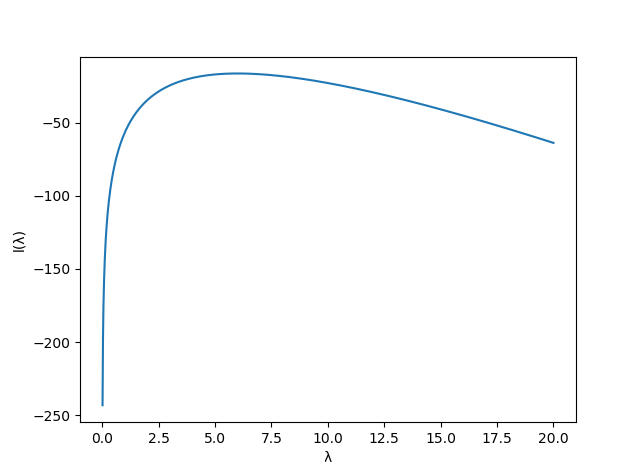
\includegraphics[width=0.5\textwidth]{1-9}
  \caption{question 1.9.}
  \label{fig:1-9}
\end{figure}

\vspace{\baselineskip}
\textit{question 1.10.}

See figure \ref{fig:1-10}.

\begin{figure}[h!]
  \centering
  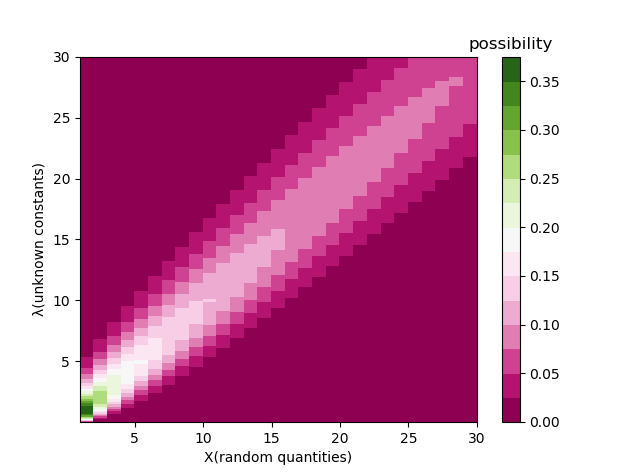
\includegraphics[width=0.5\textwidth]{1-10}
  \caption{question 1.10.}
  \label{fig:1-10}
\end{figure}

\textbf{problem 2.}

\vspace{\baselineskip}
\textit{question 2.1.}

\begin{table}[h!]
  \begin{center}
    \begin{tabular}{| c | c | c |}
      \hline
      & varibale & constant \\
      \hline
      observed& \checkmark &  \\
      \hline
      unknown &  &  \\
      \hline
    \end{tabular}
  \end{center}
  \caption{\textit{X\textsubscript{i}, ..., X\textsubscript{n}}}
\end{table}

\begin{table}[h!]
  \begin{center}
    \begin{tabular}{| c | c | c |}
      \hline
      & varibale & constant \\
      \hline
      observed&  & \checkmark \\
      \hline
      unknown &  & \\
      \hline
    \end{tabular}
  \end{center}
  \caption{\textit{x\textsubscript{i}, ..., x\textsubscript{n}}}
\end{table}

\begin{table}[h!]
  \begin{center}
    \begin{tabular}{| c | c | c |}
      \hline
      & varibale & constant \\
      \hline
      observed&  & \checkmark \\
      \hline
      unknown &  & \\
      \hline
    \end{tabular}
  \end{center}
  \caption{\textit{y\textsubscript{i}, ..., y\textsubscript{n}}}
\end{table}

\begin{table}[h!]
  \begin{center}
    \begin{tabular}{| c | c | c |}
      \hline
      & varibale & constant \\
      \hline
      observed&  &  \\
      \hline
      unknown & & \checkmark\\
      \hline
    \end{tabular}
  \end{center}
  \caption{\textit{$v$}}
\end{table}

\begin{table}[h!]
  \begin{center}
    \begin{tabular}{| c | c | c |}
      \hline
      & varibale & constant \\
      \hline
      observed&  & \checkmark \\
      \hline
      unknown &  &  \\
      \hline
    \end{tabular}
  \end{center}
  \caption{\textit{n}}
\end{table}

\vspace{\baselineskip}
\textit{question 2.2.}

Normalization factor for article length. More words a person has written in an article, more likely the word \textit{however} is used, so the length of an article need to be normalized.

\vspace{\baselineskip}
\textit{question 2.3.}

A constant to fit the Poission Distribution model.

\vspace{\baselineskip}
\textit{question 2.4.}
$p(X_i=x_i|y_i,\nu,1000) = \frac{{(\frac{\nu y_i}{1000})}^{x_i}e^{-(\frac{\nu y_i}{1000})}}{x_i!}$

\vspace{\baselineskip}
\textit{question 2.5.}
$L(y_i,\nu,1000)=p(X_i|y_i,\nu,1000)=\frac{{(\frac{\nu y_i}{1000})}^{X_i}e^{-(\frac{\nu y_i}{1000})}}{X_i!}$

\vspace{\baselineskip}
\textit{question 2.6.}

$$L(\nu)=\prod_{i=1}^np(X_i|y_i,\nu,1000)=\prod_{i=1}^n\frac{{(\frac{\nu y_i}{1000})}^{X_i}e^{-(\frac{\nu y_i}{1000})}}{X_i!}$$

\vspace{\baselineskip}
\textit{question 2.7.}

$$l(\nu)=log(L(\nu))=\sum_{i=1}^nlog(\frac{{(\frac{\nu y_i}{1000})}^{X_i}e^{-(\frac{\nu y_i}{1000})}}{X_i!})=
\sum_{i=1}^n(X_ilog(\frac{\nu y_i}{1000}) - \frac{\nu y_i}{1000} - log(X_i!))$$

\vspace{\baselineskip}
\textit{question 2.8.}

191, 93, 182, 104, 96

\vspace{\baselineskip}
\textit{question 2.9.}

$l(\nu)=$
$(191log(1.73\nu) - 1.73\nu - log(191!))$ + 
$(93log(0.947\nu) - 0.947\nu - log(93!))$ +
$(182log(1.83\nu) - 1.83\nu - log(182!))$ +
$(104log(1.21\nu) - 1.21\nu - log(104!))$ +
$(96log(1.1\nu) - 1.1\nu - log(96!))$

\vspace{\baselineskip}
\textit{question 2.10.}

As shown by figure \ref{fig:1-9}, the $lambda$ value of maximum likelihood is 6.

\begin{figure}[h!]
  \centering
  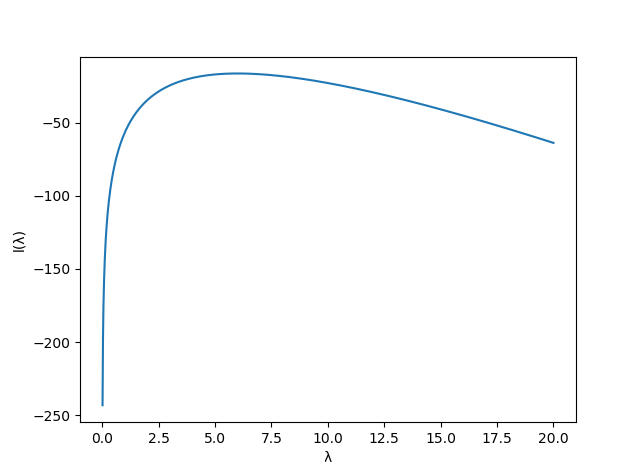
\includegraphics[width=0.5\textwidth]{1-9}
  \caption{question 1.9.}
  \label{fig:1-9}
\end{figure}

\vspace{\baselineskip}
\textit{question 1.10.}

See figure \ref{fig:1-10}.

\begin{figure}[h!]
  \centering
  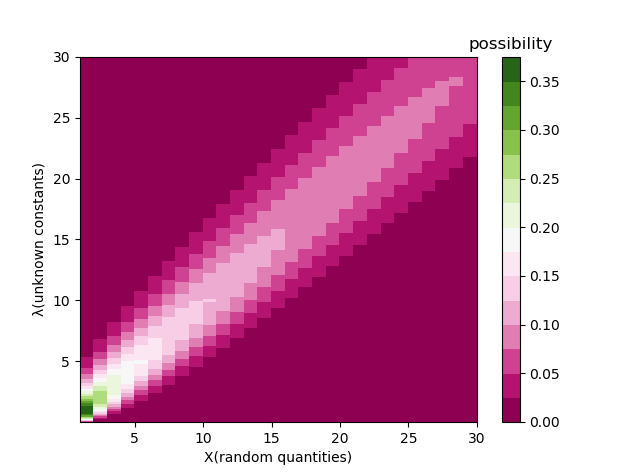
\includegraphics[width=0.5\textwidth]{1-10}
  \caption{question 1.10.}
  \label{fig:1-10}
\end{figure}

\end{document}

